\documentclass[a4paper,12pt,fleqn,oneside]{article}
\usepackage{etex}
\usepackage[latin9]{inputenc}
\usepackage{ae,aecompl}
\usepackage[T1]{fontenc}
\usepackage{ngerman}
\usepackage{fleqn}
\usepackage{ulem}
\usepackage{amssymb}
\usepackage{tabularx}
\usepackage{bm}
\usepackage{color}
\usepackage{pictex}
\usepackage[left=2.5cm,right=2.5cm,top=2cm,bottom=2cm,includeheadfoot]{geometry}
\usepackage[section]{placeins}
\usepackage{xspace}
\usepackage{multirow}
\usepackage{lastpage}
\usepackage{fancyhdr}
\usepackage{graphicx}
\usepackage{esvect}
\usepackage{textcomp}
\usepackage{amssymb}
\usepackage{fixltx2e }
\usepackage{graphicx}
\usepackage{tikz}
\usetikzlibrary{arrows}
\usepackage{siunitx}
\usepackage{pgf}
\usepackage{mathrsfs}
\usepackage{booktabs}

\sisetup{
   output-decimal-marker = {,}
}

\setlength{\headheight}{15pt}
\pagestyle{fancy}
\fancyfoot[C]{Seite \thepage{} von \pageref{LastPage}}
\linespread{1.7}
\author{Dominik Eisele}
\title{Dokumentation zur GFS "`Newton-Verfahren"'}
\date{\today}

\Huge

\newcolumntype{L}[1]{>{\raggedright\arraybackslash}p{#1}}
\newcolumntype{C}[1]{>{\centering\arraybackslash}p{#1}}
\newcolumntype{R}[1]{>{\raggedleft\arraybackslash}p{#1}}

\definecolor{dkgreen}{rgb}{0,0.6,0}
\definecolor{gray}{rgb}{0.5,0.5,0.5}
\definecolor{mauve}{rgb}{0.58,0,0.82}
\definecolor{ffqqqq}{rgb}{255,0,0}


\setlength{\tabcolsep}{0pt}
\renewcommand{\arraystretch}{1}

%\renewcommand*\contentsname{Gliederung}

\let\oldsqrt\sqrt
\def\sqrt{\mathpalette\DHLhksqrt}
\def\DHLhksqrt#1#2{\setbox0=\hbox{$#1\oldsqrt{#2\,}$}\dimen0=\ht0
\advance\dimen0-0.3\ht0
\setbox2=\hbox{\vrule height\ht0 depth -\dimen0}
{\box0\lower0.4pt\box2}}

\begin{document}

\normalem

\begin{titlepage}
	\maketitle
\end{titlepage}

\tableofcontents

\newpage

\section{Allgemeine Informationen}
	\subsection{Geschichte}
		Das Newton-Verfahren, oder auch Newton-Raphson-Verfahren, genannte Verfahren wurde nach den beiden englischen Mathematikern Sir 
		Isaac Newton (1643 - 1727) und Joseph Raphson (1648 1715) benannt. Newton veröffentlichte das Verfahren 1736 in seinem Buch
		"`Methodus fluxionum et serierum infinitarum"'. Raphson veröffentlichte eine abgewandelte Form, speziell im Bezug auf das Lösen von
		Gleichungen und Wurzeln.
 		\footnote{de.wikipedia.org/wiki/Newton-Verfahren}
		
	\subsection{Ziel des Newton-Verfahrens}
		Das Ziel des Newton-Verfahrens ist die Lösung von nichtlinearen Gleichungen der Form $f(x) = 0$. Dies geschieht über eine Linearisierung der
		Funktion. Über diese Linearisierung kann man sich nach und nach an die Nullstelle annähern.\\
		Das Verfahren ist ein Annäherungsverfahren, bei dem sich die Genauigkeit pro Wiederholung des Verfahrens ungefähr verdoppelt.
		\footnote{de.wikipedia.org/wiki/Newton-Verfahren}
		\footnote{Practical Numerical Training UKNum Nullstellenbestimmung (roots), PD. Dr. C. Mordasini Max Planck Institute for Astronomy, Heidelberg}
		
\newpage

\section{Graphische Herleitung}
	
	\subsection{Vorgehen zur Konstruktion}
		Um sich durch Konstruktion an die Nullstelle einer Funktion $f(x) = 0$ anzunähern, so muss man eine beliebige Abszisse als Startwert $x_0$
		wählen. Es ist günstig diesen Wert $x_0$ in der Nähe der zu ermittelnden Nullstelle zu wählen, um die Wahrscheinlichkeit eines möglicherweise
		auftretenden Fehlers zu minimieren. Hat man den Startwert $x_0$ ermittelt, so muss man den dazugehörigen Funktionswert $f(x)$ an der Stelle
		$x_0$ ermitteln. Man legt nun an die Funktion $f(x) = 0$ im Punkt $P(x_0|f(x))$ eine Tangente an. Nun behandelt man die Stelle $x_1$, an der
		die Tangente die x-Achse schneidet, wie die Stelle $x_0$ im vorrausgegangenen Schritt. Die Nullstelle der neu entstandenen, zweiten Tangente
		ist nun eine bessere Näherung an die Nullstelle, und gleichzeitig auch $x_2$. Dieses Verfahren wiederholt man so oft bis man die gewünschte
		Genauigkeit erreicht hat.
		\footnote{hs-esslingen.de/fileadmin/medien/mitarbeiter/koch/\\numerische\_methoden\_skript.pdf}
		\footnote{Practical Numerical Training UKNum Nullstellenbestimmung (roots), PD. Dr. C. Mordasini Max Planck Institute for Astronomy, Heidelberg}
		
\newpage

	\subsection{Graphische Herleitung}
		Zur Nullstellenbestimmung der Funktion $f(x) = \num{0.5}x^3 - 2x^2 + \num{0.5}x + 2$ (rot) wurde als Startwert $x_0 = \num{-1.6029}$
		gewählt. An dem Punkt $P(\num{-1.6029}|\num{-6})$ wurde eine Tangente (grün) an die Funktion $f(x)$ angelegt. Die Nullstelle der Tangente
		entspricht $x_1 = \num{-1.0456}$, welche eine bessere Näherung an die Nullstelle ist, als der Startwert $x_0$. Die Nullstellen der weiteren
		Tangenten (siehe Tabelle \ref{tab:nullstelle}) sind eine immer besser werdende Annäherung an die Nullstelle der Funktion.
		
		\begin{figure}[h!]
		\scalebox{1.8}{
				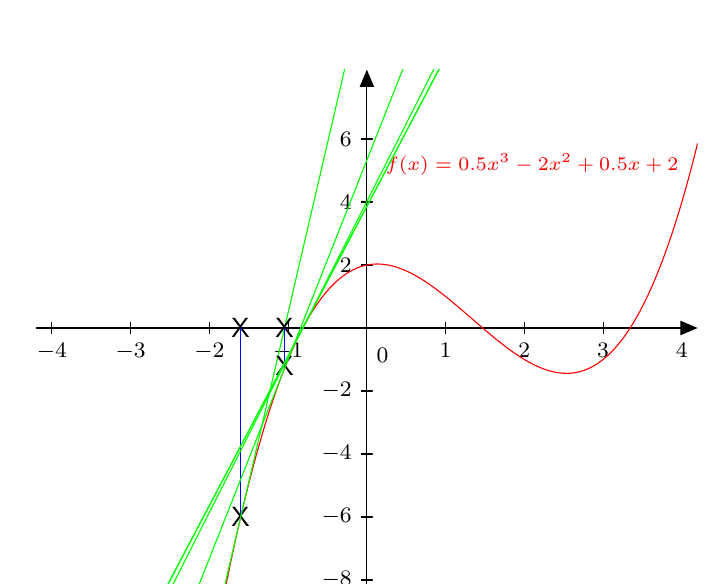
\begin{tikzpicture}[line cap=round,line join=round,>=triangle 45,x=1.0cm,y=0.4cm]
					\draw[->,color=black] (-4.2,0.) -- (4.2,0.);
					
					\foreach \x in {-4,-3,...,-1,1,2,...,4}
					\draw[shift={(\x,0)},color=black] (0pt,2pt) -- (0pt,-2pt) node[below] {\footnotesize $\x$};
					
					\draw[->,color=black] (0,-8.2) -- (0,8.2);
					
					\foreach \y in {-8,-6,...,-2,2,4,6}
					\draw[shift={(0,\y)},color=black] (2pt,0pt) -- (-2pt,0pt) node[left] {\footnotesize $\y$};
							
					\draw[color=black] (0pt,-10pt) node[right] {\footnotesize $0$};
					
					\clip(-4.2,-8.2) rectangle (4.2,8.2);
					
					\draw[color=red,smooth,samples=100,domain=-4.2:4.2] plot(\x,{0.5*(\x)^(3.0)-2.0*(\x)^(2.0)+0.5*(\x)+2.0});
					
					\begin{scriptsize}
						\draw[color=ffqqqq] (2.1,5.2) node {$f(x) = \num{0.5}x^3 - 2x^2 + \num{0.5}x + 2$};
					\end{scriptsize}
					
					\node (1) at (-1.603,0) {\textsf{X}};
					
					\draw [blue] (-1.603,0) -- (-1.603,-6);
			
					\node (2) at (-1.60298,-6) {\textsf{X}};
					
					\draw[color=green,smooth,samples=100,domain=-4.2:4.2] plot(\x,{10.76624*\x+11.25802});
					
					\node (3) at (-1.04568,0) {\textsf{X}};	
					
					\draw [blue] (-1.04568,0) -- (-1.04568,-1.21842);	
					
					\node (4) at (-1.04568,-1.21842) {\textsf{X}};
					
					\draw[color=green,smooth,samples=100,domain=-4.2:4.2] plot(\x,{6.32288*\x+5.33027});
					
					\draw[color=green,smooth,samples=100,domain=-4.2:4.2] plot(\x,{4.93807*\x+4.02045});
					
					\draw[color=green,smooth,samples=100,domain=-4.2:4.2] plot(\x,{4.75103*\x+3.86547});
					
					\draw[color=green,smooth,samples=100,domain=-4.2:4.2] plot(\x,{4.74736*\x+3.86248});
				\end{tikzpicture}
			} 
		\end{figure}
		
\FloatBarrier
		\begin{table}[]
			\centering
			\begin{tabular}{@{}ll@{}}
				\toprule
				Berechnungsschritt\ \ \ \ 		& Abszissenwert \\ \midrule
				0                  				& -1,6029       \\
				1                  				& -1,0456       \\
				2                  				& -0,8430       \\
				3                  				& -0,8141       \\
				4                  				& -0,8136       \\
				5                  				& -0,8136       \\
				Berechneter Wert   			& -0,8136       \\ \bottomrule
			\end{tabular}
			\caption{Annäherrung an die Nullstelle}
			\label{tab:nullstelle}
		\end{table}
		
\FloatBarrier
		
		\noindent
		Die in Tabelle \ref{tab:nullstelle} zu sehenden Werte sind die Nullstellen in Abhängigkeit des Berechnungsschrittes. Zwischen den Werten von
		Berechnungsschritt vier und fünf ist keine Veränderung mehr zu sehen. Das bedeutet, dass der Wert, auf vier Stellen gerundet, exakt ist.
		Weitere Veränderungen finden ab hier nur noch ab der fünften Nachkommastelle statt. Das graphisch ermittelte Ergebnis stimmt auch mit dem
		berechneten Wert von \num{-0.8136} überein.

\newpage

\section{Berechnung}
	\subsection{Iterationsformel}
		\ \ 
		{\fboxsep=.2in $$\framebox{$x_{n+1} = x_{n} - \frac{f(x_{n})}{f^\prime(x_{n})}$}$$}\ \ 
		 
		Um Nullstellen einer Gleichung mit dem Newton-Verfahren zu lösen benötigt man die Iterationsformel (von lat. iterare "`wiederholen"').
		Um die Nullstelle mit dieser Formel zu berechnen, benötigt man die zu lösende Funktion $f(x)$, sowie deren Ableitung $f^\prime(x)$ und einen
		Startwert $x_0$. Um nun $x_1$ zu erhalten muss man $x_0$ in die Formel einsetzen. Der nun entstandene Wert $x_1$ ist die Annäherung an
		die Nullstelle. Benötigt man eine höhere Genauigkeit, so muss man $x_1$ erneut in die Formel einsetzen, bzw. die Iteration so lange durchführen
		bis die gewünschte Genauigkeit erreicht ist.

	\subsection{Herleitung}
		Das Ziel des Newton-Verfahrens ist es die Nullstelle der Tangente zu berechnen. Da diese eine Gerade ist gilt die allgemeine Geradengleichung:
		$y = mx + b$. Da man die Tangente an die Stelle der Funktion anlegt, deren Abszisse $x_0$ und der Funktionswert $f(x_0)$ ist, ergibt sich ein Punkt
		$P$ auf der Tangente, der die Koordinaten $P(x_0|f(x_0))$ besitzt. Da die Tangente im Berührpunkt $P$ an die Funktion angelegt wurde, besitzt
		sie an Punkt $P$ dieselbe Steigung wie die Funktion $f(x)$, d.\,h. die Steigung der Tangente ist $f^\prime(x)$.\\
		Setzt man diese Werte nun in die Geradengleichung ein, so ergibt sich die Gleichung $f(x_0) = f^\prime(x_0) \cdot x_0  + b$. Stellt man diese
		nun nach $b$ um, so ergibt sich für $b$ die Gleichung $b = f(x_0) - f^\prime(x_0) \cdot x_0$.\\
		Setzt man nun erneut alle Werte in die Geradengleichung ein, so erhält man folgende Geradengleichung für die Tangente:
		$y = f^\prime(x_0) \cdot x  + f(x_0) - f^\prime(x_0) \cdot x_0$. Um die Nullstelle der Gleichung zu bestimmen setzt man die Gleichung gleich
		Null. So erhält man die Gleichung $0 = f^\prime(x_0) \cdot x_1  + f(x_0) - f^\prime(x_0) \cdot x_0$. Formt man diese nun nach $x$ um, so
		erhält man die Iterationsformel $x_1 =x_0 - \frac{f(x_0)}{f^\prime(x_0)}$.
		\footnote{hs-esslingen.de/fileadmin/medien/mitarbeiter/koch/\\numerische\_methoden\_skript.pdf}
	
\newpage
		
\section{Fazit}
	\subsection{Vorteile des Newton-Verfahrens}
		Beim Newton-Verfahren ist eine schnelle Konvergenz möglich, da sich die Anzahl an signifikanten Stellen pro Iterationsschritt ungefähr verdoppelt.
		Dabei ist nur ein Startwert ($x_0$) nötig um eine Konvergenz zu erzielen. Die Nachteile und Probleme die entstehen können, sind durch eine
		bessere Wahl des Startwerts vermeidbar.\\
		Dabei sollte beachtet werden, dass in der Praxis der Einsatz vom Newton-Verfahren ungeeignet ist. Zur sicheren Verwendung benötigt man eine
		Mischform mit einem anderen Verfahren, sodass eine günstige Wahl des Startpunktes ermöglicht wird.
		\footnote{Practical Numerical Training UKNum Nullstellenbestimmung (roots), PD. Dr. C. Mordasini Max Planck Institute for Astronomy, Heidelberg}
	
	\subsection{Nachteile des Newton-Verfahrens}
		Beim Newton-Verfahren ist keine Konvergenz garantiert. So kann es vorkommen dass, für ein $x_0$ in der Nähe von Sattelstellen oder auf
		Sattelstellen die Tangente parallel zur x-Achse verläuft, oder die Steigung minimal ist so dass der Schnittpunkt sehr weit entfernt von der
		Nullstelle ist. Dies ist in Abbildung \ref{fig:sattelstelle} zu sehen.\\
		In Abbildung \ref{fig:ring} ist ein nichtkonvergenter Zyklus zu sehen. Bei so einem Zyklus rotieren die Werte immer und es gibt keine Nullstelle.
		Dies ist der Fall, wenn die Nullstelle einer Tangente gleich einem anderen Wert von $x_n$ ist.\\
		Hat man eine oszillierende  Funktion, oder eine Funktion mit mehreren Nullstellen, so kann es passieren, dass sich das Newton-Verfahren an eine
		Nullstelle annähert, die deutlich weiter vom Startwert entfernt ist als eine andere.\\
		All diese Fehler können durch einen anderen Startwert umgangen werden.
		\footnote{Practical Numerical Training UKNum Nullstellenbestimmung (roots), PD. Dr. C. Mordasini Max Planck Institute for Astronomy, Heidelberg}

		\begin{figure}
			\centering
			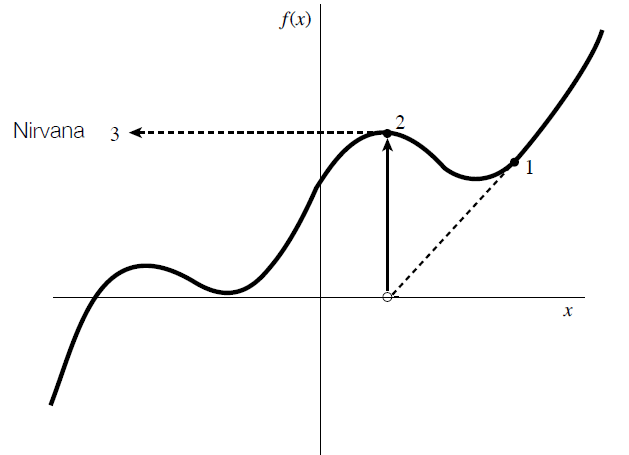
\includegraphics[width=0.5\linewidth]{Sattelstelle.png}
			\caption{Sattelpunkt}
			\label{fig:sattelstelle}
		\end{figure}
		
		\begin{figure}
			\centering
			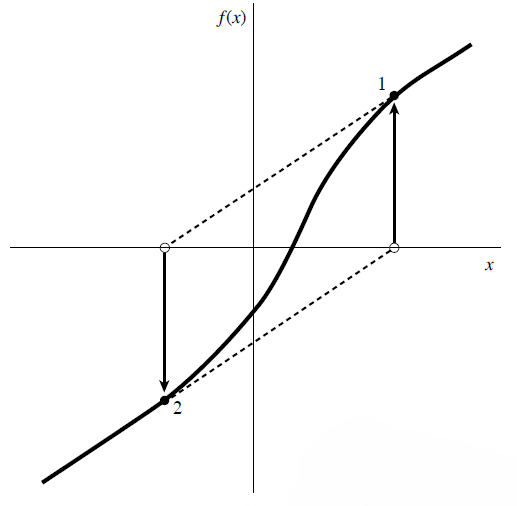
\includegraphics[width=0.5\linewidth]{Ring.png}
			\caption{Zyklus}
			\label{fig:ring}
		\end{figure}
		
		\begin{figure}
			\centering
			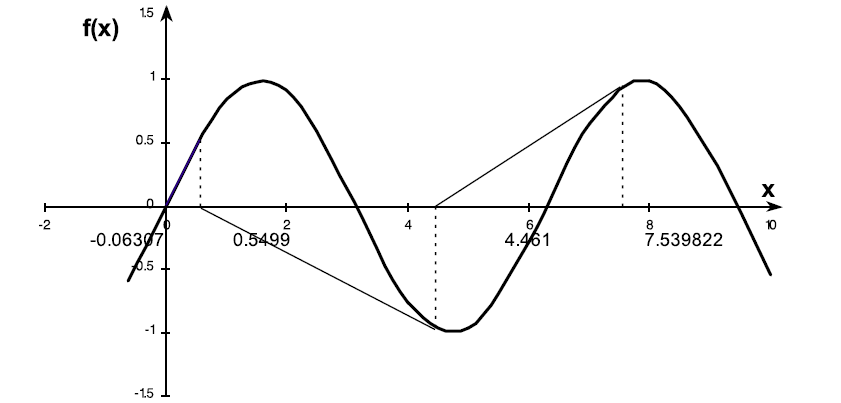
\includegraphics[width=0.5\linewidth]{hupfen.png}
			\caption{Nullstellenspringen}
			\label{fig:hupfen}
		\end{figure}

\newpage

\section{Kehrwertberechnung}

	Bei Schaltungen mit schnellen Multiplizierern kann es von Vorteil sein, wenn man anstatt zu dividieren mit dem Kehrbruch multipliziert. Den Kehrwert
	für dieses Verfahren kann man mit dem Newton Verfahren berechnen. Um den Kehrwert von $A$ zu berechnen kann man die Formel $x = \frac{1}{A}$
	aufstellen, dabei ist $x$ der gesuchte Kehrwert. Um das Newton-Verfahren anwenden zu können, muss man die Formel auf die Form $f(x) = 0$ bringen.
	Wenn man die Gleichung nun umformt, so erhält man $0 = \frac{1}{x} - A$. Die Nullstelle von $f(x) = \frac{1}{x} - A$ ist somit der Kehrwert von $A$.
	Um die Funktion in die Iterationsformel einsetzten zu können, muss man sie ableiten. Daraus ergibt sich $f^\prime(x) = -\frac{1}{x²}$. Setzt man diese
	Funktionen nun in die Gleichung ein, so ergibt sich als Iterationsfunktion \\$f(x) = x- \frac{\frac{1}{x} - A}{-\frac{1}{x²}}$. Stellt man dies nun um, so hat
	man $f(x) = x \cdot (2 - A \cdot x)$ als Iterationsfunktion zur Berechnung des Kehrwerts.

\newpage

\section{Quellen}
	\begin{itemize}
		\item An Accurate, High Speed Implementation of Division by Reciprocal Approximation, D.L. Fowler and J.E. Smith, Astronautics Corperation of
			Amerika
		\item Floating-Point IP Cores User Guide
		\item Practical Numerical Training UKNum Nullstellenbestimmung (roots), PD. Dr. C. Mordasini Max Planck Institute for Astronomy, Heidelberg
		\item Rechnerarithmetik Thema: Iterative Division, Quadratwurzelberechnung, Eberhard Zehendner, Friedrich-Schiller-Universität Jena
		\item hs-esslingen.de/fileadmin/medien/mitarbeiter/koch/\\numerische\_methoden\_skript.pdf (Abgerufen: 08.01.2017, 12:10 Uhr)
		\item de.wikipedia.org/wiki/Newton-Verfahren (Abgerufen: 08.01.2017, 12:10 Uhr)
	\end{itemize}

\end{document}
